% Beamer presentation, 16:9.
% Each slide is a frame. \pause and overlays like <2-> reveal content step by step.
\documentclass[aspectratio=169,11pt]{beamer} % aspectratio=43 for 4:3 projectors

% ---- Look ---------------------------------------------------------------------
% Try other themes: \usetheme{Madrid}, {Berlin}, {Singapore}; colour themes: {beaver}, {crane}.
\usetheme{default}
\definecolor{accent}{RGB}{91,77,200} % change the accent colour here
\setbeamercolor{structure}{fg=accent}
\setbeamercolor{title}{fg=accent}
\setbeamercolor{frametitle}{fg=accent}
\setbeamercolor{block title}{bg=accent!15,fg=accent!70!black}
\setbeamercolor{block body}{bg=accent!5}
\setbeamertemplate{blocks}[rounded][shadow=false]
\setbeamertemplate{navigation symbols}{}        % hide the navigation icons
\setbeamertemplate{footline}[frame number]      % slide numbers bottom right
\setbeamerfont{title}{series=\bfseries}
\setbeamerfont{frametitle}{series=\bfseries}

\usepackage[english]{babel}
\usepackage{booktabs}
\usepackage{tikz}

\usepackage[style=authoryear,backend=biber]{biblatex}
\addbibresource{references.bib}
\usepackage{csquotes}

\title{Title of Your Talk}
\subtitle{An optional subtitle}
\author{Speaker Name}
\institute{Your Institution}
\date{Conference or Seminar, \today}

\begin{document}

\begin{frame}
  \titlepage
\end{frame}

\begin{frame}{Outline}
  \tableofcontents
\end{frame}

\section{Motivation}

\begin{frame}{The question}
  \begin{itemize}
    \item Start with why the audience should care.
    \pause
    \item Then reveal one point at a time with \texttt{\textbackslash pause}.
    \pause
    \item Keep it to a few words per line.
  \end{itemize}
\end{frame}

\section{Approach}

\begin{frame}{Two columns}
  \begin{columns}[T]
    \begin{column}{0.48\textwidth}
      \begin{block}{Idea}
        Put the key message in a block.
      \end{block}
      \begin{alertblock}{Watch out}
        Alert blocks draw attention.
      \end{alertblock}
    \end{column}
    \begin{column}{0.48\textwidth}
      \centering
      % Replace with \includegraphics[width=\linewidth]{figure.png}
      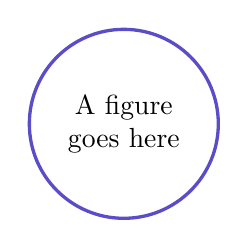
\begin{tikzpicture}
        \draw[accent,very thick] (0,0) circle (1.2);
        \node[align=center] {A figure\\goes here};
      \end{tikzpicture}
    \end{column}
  \end{columns}
\end{frame}

\begin{frame}{Equations and tables}
  \[
    \hat{\theta} = \arg\min_{\theta} \sum_{i=1}^{n} \bigl(y_i - f(x_i;\theta)\bigr)^2
  \]
  \begin{center}
    \begin{tabular}{lr}
      \toprule
      Method & Score \\
      \midrule
      Before & 0.71 \\
      After  & \alert{0.84} \\
      \bottomrule
    \end{tabular}
  \end{center}
\end{frame}

\section{Conclusion}

\begin{frame}{Take-home message}
  \begin{enumerate}
    \item<1-> The one thing to remember.
    \item<2-> The second thing.
  \end{enumerate}
  \vfill
  \small Builds on \textcite{knuth1984}.
\end{frame}

\begin{frame}{References}
  \printbibliography[heading=none]
\end{frame}

\begin{frame}[plain]
  \centering\Huge Thank you!\par\bigskip
  \normalsize Questions? \texttt{speaker@example.org}
\end{frame}

\end{document}
